\documentclass[sigplan,screen]{acmart}



% Add these lines to disable ACM Reference Format 
\settopmatter{printacmref=false} % Remove ACM Reference Format



%% \BibTeX command to typeset BibTeX logo in the docs
\AtBeginDocument{%
  \providecommand\BibTeX{{%
    Bib\TeX}}}

%% Rights management information.  This information is sent to you
%% when you complete the rights form.  These commands have SAMPLE
%% values in them; it is your responsibility as an author to replace
%% the commands and values with those provided to you when you
%% complete the rights form.
%% Customize the rights management information
\setcopyright{acmlicensed} % or choose an appropriate option like 'acmlicensed', 'rightsretained', etc.
\acmConference[Conference'17]{Conference on Great Research}{June 2024}{Tehran, Iran}
\acmYear{2024}
\copyrightyear{2024}
\acmDOI{10.1145/1234567.8901234}



%%
%%  Uncomment \acmBooktitle if the title of the proceedings is different
%%  from ``Proceedings of ...''!
%%
%%  \acmBooktitle{Woodstock '18: ACM Symposium on Neural Gaze Detection,
%%  June 03--05, 2018, Woodstock, NY}
\acmISBN{978-1-4503-1234-5/24/06}



%%
%% Submission ID.
%% Use this when submitting an article to a sponsored event. You'll
%% receive a unique submission ID from the organizers
%% of the event, and this ID should be used as the parameter to this command.
%%\acmSubmissionID{123-A56-BU3}

%%
%% For managing citations, it is recommended to use bibliography
%% files in BibTeX format.
%%
%% You can then either use BibTeX with the ACM-Reference-Format style,
%% or BibLaTeX with the acmnumeric or acmauthoryear sytles, that include
%% support for advanced citation of software artefact from the
%% biblatex-software package, also separately available on CTAN.
%%
%% Look at the sample-*-biblatex.tex files for templates showcasing
%% the biblatex styles.
%%

%%
%% The majority of ACM publications use numbered citations and
%% references.  The command \citestyle{authoryear} switches to the
%% "author year" style.
%%
%% If you are preparing content for an event
%% sponsored by ACM SIGGRAPH, you must use the "author year" style of
%% citations and references.
%% Uncommenting
%% the next command will enable that style.
%% \citestyle{acmauthoryear}


%%
%% end of the preamble, start of the body of the document source.

\usepackage{amsmath}  % For mathematical symbols and environments
\usepackage{algorithm}  % For algorithm environment
\usepackage{algpseudocode}  % For algorithmic pseudocode
\usepackage{tikz}  % For drawing diagrams
\usepackage{caption}
\usepackage{algorithmicx}
\usepackage{amsfonts}
\usepackage{float} % Add this line to include the float package
\usetikzlibrary{calc}
\usetikzlibrary{matrix}
\usetikzlibrary{shapes.multipart, shapes, arrows}



% Redefine the algorithmic keywords to remove "Function" and "EndFunction"
\floatname{algorithm}{}
\renewcommand{\thealgorithm}{}

%----------------------------------------------------

% xintfrac does not load xinttools, this must be done explicitely if needed as here.
\usepackage{xintfrac, xinttools}
\usepackage{tikz}

%----------------------------------------------------------------

% FIRST PART: TikZ styles and macros for the actual drawing
\newcounter{cellcount}%  used for coordinates of the node
\newcounter{pivotcount}% when it will remain at zero, will signal the sort is finished.

% Styles defined by Tom Bombaldi. (modified: all share the same size)
% (re-modified \bf -> \bfseries due to extremely annoying warnings from
% KOMA-script which are truly a pain and do not make any sense regarding \bf:
% if I want to use \bf, and know what I am doing, why should I get HARASSED
% by police of LaTeX good conduct ? )
\tikzset{l/.style={minimum width=6mm, minimum height=6mm, rounded corners=1.5mm, draw=black, fill=lime!70!gray},
        o/.style={minimum width=6mm, minimum height=6mm, rounded corners=1.5mm, draw=black, fill=olive!50},
        r/.style={minimum width=6mm, minimum height=6mm, rounded corners=1.5mm, draw=black, fill=magenta!50!black, text=white, font=\bfseries, yshift=1.5mm},
% this is the "b" style as used in the image below
%        b/.style={minimum width=6mm, minimum height=6mm, rounded corners=1.5mm, draw=black, fill=magenta!50!black, text=white, font=\bfseries},
% nicer:
        b/.style={minimum width=6mm, minimum height=6mm, rounded corners=1.5mm, draw=black, fill=white, text=magenta!50!black, font=\bfseries},
        g/.style={minimum width=6mm, minimum height=6mm, rounded corners=1.5mm, draw=black, fill=gray, text=white, font=\bfseries}}

% NOTE the b style was originally the same as the r(aised) style apart from
% not being raised, but I find it nicer with a somewhat different
% specification. I have not updated the images though.

% How the nodes are drawn depending on whether on the left of the pivot value
% or on the right, or is a pivot value, or a raised pivot during selection phase.

\def\DecoLEFT #1{%
   \xintFor* ##1 in {#1} \do 
   {\stepcounter{cellcount}\node[o] at (\arabic{cellcount},0) {##1};}%
}

\def\DecoINERT #1{%
   \xintFor* ##1 in {#1} \do 
   {\stepcounter{cellcount}\node[g] at (\arabic{cellcount},0) {##1};}%
}

\def\DecoRIGHT #1{%
   \xintFor* ##1 in {#1} \do 
   {\stepcounter{cellcount}\node[l] at (\arabic{cellcount},0) {##1};}%
}

\def\DecoLEFTwithPivot #1{\stepcounter{pivotcount}%
     \xintFor* ##1 in {#1} \do 
     {\stepcounter{cellcount}%
      \xintifForLast {\node[r]}{\node[o]} at (\arabic{cellcount},0) {##1};}%
}

\def\DecoINERTwithPivot #1{\stepcounter{pivotcount}%
     \xintFor* ##1 in {#1} \do 
     {\stepcounter{cellcount}%
      \xintifForLast {\node[b]}{\node[g]} at (\arabic{cellcount},0) {##1};}%
}

\def\DecoRIGHTwithPivot #1{\stepcounter{pivotcount}%
     \xintFor* ##1 in {#1} \do 
     {\stepcounter{cellcount}%
      \xintifForLast {\node[r]}{\node[l]} at (\arabic{cellcount},0) {##1};}%
}

%----------------------------------------------------------------
% SECOND PART: the actual sorting routines.

\makeatletter
\def\QS@sort@a #1{\expandafter \QS@sort@b \expandafter {\xintLength {#1}}{#1}}
\def\QS@sort@b #1{\ifcase #1
                      \expandafter\QS@sort@empty
                   \or\expandafter\QS@sort@single
                 \else\expandafter\QS@sort@c
                 \fi
}%
\def\QS@sort@empty  #1{}
\def\QS@sort@single #1{\QSIr {#1}}

% This step is to pick the last as pivot.
\def\QS@sort@c #1%
   {\expandafter\QS@sort@d\expandafter {\romannumeral0\xintnthelt {-1}{#1}}{#1}}%

% Here \QSLr, \QSIr, \QSr have been let to \relax.
% The trick with \xintApplyUnbraced is that for example when selecting
% the elements smaller than pivot, if we had been using \xintApply we 
% would have had at the minimum an empty brace pair. Thus we use the
% "unbraced" variant, but then the \QS@select@smaller has added in
% anticipation a level of braces.
\def\QS@sort@d #1#2{%
    \QSLr {\xintApplyUnbraced {\QS@select@smaller  {#1}}{#2}}%
    \QSIr {\xintApplyUnbraced {\QS@select@equal    {#1}}{#2}}%
    \QSRr {\xintApplyUnbraced {\QS@select@greater {#1}}{#2}}%
}%
\def\QS@select@smaller #1#2{\xintifLt {#2}{#1}{{#2}}{ }}% space will stop a f-expansion
\def\QS@select@equal   #1#2{\xintifEq {#2}{#1}{{#2}}{ }}% space will stop a f-expansion
\def\QS@select@greater #1#2{\xintifGt {#2}{#1}{{#2}}{ }}% space will stop a f-expansion

\makeatother
%
% NOTE 1: thus, each comparison with the pivot is done three (!) times.
%
% NOTE 2: we may well end up with \QSLr {<empty>} situations. THis is handled
% silently by the \xintFor loops, and also when \QSLr becomes \QS@sort@a, the
% latter must handle correctly an empty argument.

%----------------------------------------------------------------
% THIRD PART: the main macros \QSpivotStep, \QSsortStep and \QSinitialize.

\makeatletter
% This draws all with suitable highlighting for the newly chosen pivots
% (which will be shown raised)
\def\QSpivotStep {\let\QSLr\DecoLEFTwithPivot
                \let\QSIr\DecoINERT
                \let\QSIrr\DecoINERT
                \let\QSRr\DecoRIGHTwithPivot
\par\centerline{\rule[1.5mm]{0pt}{8mm}%
            \setcounter{cellcount}{0}\setcounter{pivotcount}{0}%
            \begin{tikzpicture}\QS@list\end{tikzpicture}}
}

% This sorts and then draws, showing where the pivot chosen in the previous
% step go. Next time they will have become "inert". If pivotcount is still at
% zero on exit from \QSpivotStep, then this is the signal to stop before
% executing \QSsortStep.
\def\QSsortStep {\def\QSLr {\noexpand\QS@sort@a}% 
                 \def\QSRr {\noexpand\QS@sort@a}%
                 \def\QSIr {\noexpand\QSIrr}%
                 \let\QSIrr\relax
                    \edef\QS@list{\QS@list}%
                \let\QSLr\relax 
                \let\QSRr\relax
                \let\QSIr\relax
                    \edef\QS@list{\QS@list}%
                \let\QSLr\DecoLEFT
                \let\QSIr\DecoINERTwithPivot
                \let\QSIrr\DecoINERT
                \let\QSRr\DecoRIGHT
\par\centerline{\rule[1.5mm]{0pt}{8mm}%
            \setcounter{cellcount}{0}%
            \begin{tikzpicture}\QS@list\end{tikzpicture}}
}

\def\QSinitialize #1{%
    % first, we convert the comma separated values into a list of braced items
    % we use an \edef, and anyhow many \edef's will be used later
    \edef\QS@list {\noexpand\QSRr {\xintCSVtoList {#1}}}%
    \let\QSRr\DecoRIGHT
    % The \QSRr marker mutated to draw the last element as
    % pivot and the earlier ones with the suitable style.
    %
    % The list of marked braced items \QS@list is used both for drawing
    % (as here) and for doing the exchange of elements during sort.
    \par\centerline{\rule[1.5mm]{0pt}{8mm}\setcounter{cellcount}{0}%
                \begin{tikzpicture}\QS@list\end{tikzpicture}}
}
\makeatother

\begin{document}


%%
%% The "title" command has an optional parameter,
%% allowing the author to define a "short title" to be used in page headers.
\title{Sorting Algorithms}

%%
%% The "author" command and its associated commands are used to define
%% the authors and their affiliations.
%% Of note is the shared affiliation of the first two authors, and the
%% "authornote" and "authornotemark" commands
%% used to denote shared contribution to the research.




\author{Fatemeh Taghavi}
\affiliation{%
  \institution{K. N. Toosi University of Technology}
  \city{Tehran}
  \country{Iran}}
\email{taghaviiifatemeh83@gmail.com}

\author{Mobina Khaksar}
\affiliation{%
  \institution{K. N. Toosi University of Technology}
  \city{Tehran}
  \country{Iran}}
\email{mobina.khaksar4@gmail.com}

\author{Sara Ghafoury}
\affiliation{%
  \institution{K. N. Toosi University of Technology}
  \city{Tehran}
  \country{Iran}}
\email{saraghbaba83@gmail.com}

%%
%% By default, the full list of authors will be used in the page
%% headers. Often, this list is too long, and will overlap
%% other information printed in the page headers. This command allows
%% the author to define a more concise list
%% of authors' names for this purpose.
\renewcommand{\shortauthors}{Taghavi et al.}

%%
%% The abstract is a short summary of the work to be presented in the
%% article.
\begin{abstract}
  Sorting algorithms are fundamental to computer science, providing
  essential tools for organizing data efficiently. This paper explores
  and compares five widely used sorting algorithms: Insertion Sort, 
  Merge Sort, Bubble Sort, Heap Sort, and Quick Sort. We analyze each 
  algorithm's time complexity, space complexity, and performance in 
  different scenarios. Through empirical analysis and theoretical 
  discussion, this study aims to provide a comprehensive understanding 
  of these algorithms' strengths and weaknesses, helping practitioners 
  select the most appropriate sorting method for specific applications.
\end{abstract}


%%
%% Keywords. The author(s) should pick words that accurately describe
%% the work being presented. Separate the keywords with commas.
\keywords{Sorting algorithms, Insertion Sort, Merge Sort, Bubble Sort, 
Heap Sort, Quick Sort, Time complexity, Space Complexity, Algorithm Performance }
%% A "teaser" image appears between the author and affiliation
%% information and the body of the document, and typically spans the
%% page.

% \begin{comment}
% \begin{teaserfigure}
%   \includegraphics[width=\textwidth]{sampleteaser}
%   \caption{Seattle Mariners at Spring Training, 2010.}
%   \Description{Enjoying the baseball game from the third-base
%   seats. Ichiro Suzuki preparing to bat.}
%   \label{fig:teaser}
% \end{teaserfigure}
% \end{comment}

% \received{20 February 2007}
% \received[revised]{12 March 2009}
% \received[accepted]{5 June 2009}

%%
%% This command processes the author and affiliation and title
%% information and builds the first part of the formatted document.
\maketitle

\section*{Introduction}
  The history of sorting algorithms dates back to the early days of computer
  science and remains a critical area of study. Sorting is the process of
  arranging data in a specific order, typically ascending or descending.
  The efficiency of sorting algorithms directly impacts the performance of
  numerous applications, including database management, search algorithms,
  and data analysis.

  This paper focuses on five prominent sorting algorithms: Insertion Sort,
  Merge Sort, Bubble Sort, Heap Sort, and Quick Sort. These algorithms have 
  been extensively studied and applied in various domains due to their 
  unique characteristics and performance profiles. Insertion Sort, known for
  its simplicity, performs well on small or nearly sorted datasets. 
  Merge Sort, a divide-and-conquer algorithm, is stable and effective for 
  large datasets. Bubble Sort, though less efficient for large datasets, 
  is easy to implement and understand. Heap Sort, utilizing a binary heap 
  data structure, offers reliable performance without requiring additional 
  space. Quick Sort, often the fastest in practice, uses a partitioning 
  approach but can degrade in performance under certain conditions.

  The primary goal of this study is to compare these sorting algorithms 
  based on their time and space complexities, stability, and practical 
  performance across different types of datasets. By providing a detailed 
  analysis, we aim to assist software developers and computer scientists 
  in selecting the most suitable sorting algorithm for their specific needs.
  
  Our contributions include:

  \begin{itemize}
    \item A comprehensive review of the theoretical foundations of each 
    sorting algorithm.
    \item An empirical performance comparison using various datasets.
    \item A discussion on the practical considerations for choosing an 
    appropriate sorting algorithm based on specific application requirements.
  \end{itemize}

  Through this work, we hope to contribute to the ongoing research and 
  development of efficient sorting techniques, ensuring that the best 
  practices are employed in both academic and industrial settings.



\section*{Preliminaries}

  Sorting algorithms are critical to the efficiency of numerous computational 
  tasks, making their study a cornerstone of computer science. This section 
  provides the necessary background and preliminaries required to understand 
  the sorting algorithms discussed in this paper.

  \subsection{Sorting Algorithms}
  
  A sorting algorithm is a method for rearranging a list or array of elements 
  in a specific order, typically in ascending or descending numerical or 
  lexicographical order.

  \subsection{Input Array}
  
  An array $A$ of $n$ elements, where $A = [a_1, a_2, \ldots, a_n ] $,
  is provided as the input to the sorting algorithm.The goal is to transform 
  this array into a sorted array $A^\prime $ where 
  $a_1^\prime \leq  a_2^\prime\leq  \ldots \leq a_n^\prime$.

  \subsection{Comparison-Based Sorting}
  
  Most traditional sorting algorithms operate by comparing elements to 
  determine their order. The efficiency of these algorithms often depends 
  on the number of comparisons made.


  \subsection{Inversions}
  An inversion in an array is a pair of elements where the preceding element
  is greater than the following one. Inversions are used to measure how far
  an array is from being sorted. The number of inversions in an array can 
  give insights into the efficiency of sorting algorithms, especially those 
  that are comparison-based.

  Formally, given an array \( A \) of \( n \) elements, an inversion is a 
  pair of indices \( (i, j) \) such that \( i < j \) and \( A[i] > A[j] \).



  \subsection{Random Access}
  
  The input array is stored in a structure that allows random access, meaning 
  any element $a_i$ can be accessed in constant time $O(1)$.

  \subsection{Big O Notation}
  
  Big O notation, denoted as $O(f(n))$, is used to describe the upper bound 
  of an algorithm's running time. It provides an asymptotic analysis of the
  algorithm's performance, allowing us to understand how the running time 
  grows relative to the input size $n$. Formally, we say that a function 
  $T(n)$ is $O(f(n))$if there exist positive constants $c$ and $n_0$ 
  such that for all $n \geq n_0$, the following inequality holds:
  \[
  T(n) \leq c \cdot f(n)
  \]
  
  \subsection{Time Complexity}
  
  Time complexity is a measure of the amount of time an algorithm takes 
  to complete as a function of the size of the input. It helps in comparing
  the efficiency of different algorithms. Time complexities are typically 
  classified into three categories: average case, best case, and worst 
  case.
  
  \begin{itemize}
      \item \textbf{Best Case:} The scenario where the algorithm performs 
      the minimum number of operations. For sorting algorithms, this often 
      occurs when the input array is already sorted.
      \item \textbf{Average Case:} The expected time over all possible 
      inputs of size $n$. This provides a realistic measure of the 
      algorithm's performance in everyday use.
      \item \textbf{Worst Case:} The scenario where the algorithm performs 
      the maximum number of operations. This case is crucial as it provides
      an upper bound on the running time, ensuring that the algorithm will
      not exceed this time for any input.
  \end{itemize}
  
  \subsection{Space Complexity}
  
  Space complexity refers to the amount of memory an algorithm uses 
  relative to the input size. It is crucial for understanding the overall 
  resource requirements of an algorithm. Space complexity is often 
  categorized into:
  
  \begin{itemize}
      \item \textbf{In-place:} Algorithms that use a constant amount of 
      extra space, usually $O(1)$.
      \item \textbf{Not in-place:} Algorithms that require additional 
      space proportional to the input size, typically $O(n)$ or more.
  \end{itemize}


\section{Insertion Sort}
Insertion Sort is a straightforward and efficient comparison-based sorting 
algorithm. It is widely used for sorting small datasets or nearly sorted 
arrays due to its simplicity and ease of implementation. The algorithm 
operates similarly to the way humans sort playing cards, making it an 
intuitive method for understanding basic sorting principles.

Insertion Sort constructs the final sorted array one element at a time. 
It starts by assuming that the first element is already sorted. It then 
picks the next element and inserts it into the correct position relative 
to the already sorted elements. This process is repeated for each element 
until the entire array is sorted.



\begin{figure}[H]  % Use the H option to force the figure placement
  \centering
  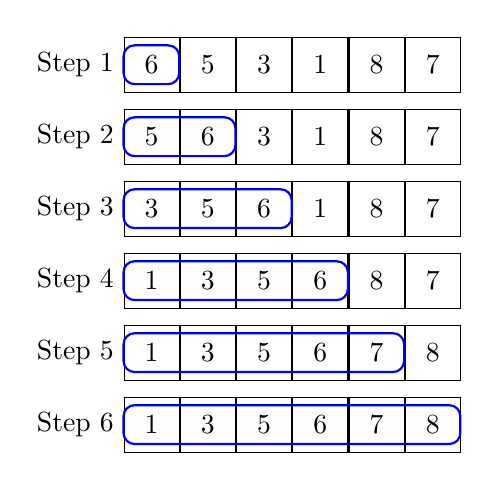
\begin{tikzpicture}
    \matrix[matrix of nodes, nodes in empty cells, nodes={draw, minimum size=7mm, anchor=center}, column sep=0mm, row sep=2mm] (m) {
      6 & 5 & 3 & 1 & 8 & 7 \\
      5 & 6 & 3 & 1 & 8 & 7 \\
      3 & 5 & 6 & 1 & 8 & 7 \\
      1 & 3 & 5 & 6 & 8 & 7 \\
      1 & 3 & 5 & 6 & 7 & 8 \\
      1 & 3 & 5 & 6 & 7 & 8 \\
    };
    
    % Label rows with step numbers
    \foreach \i in {1,...,6}
      \node[anchor=east] at (m-\i-1.west) {Step \i};

    % Highlight sorted part with centered blue squares
    \foreach \i/\j in {1/1, 2/2, 3/3, 4/4, 5/5, 6/6} {
      \draw[rounded corners, blue, thick] 
      ([yshift=-6mm] m-\i-1.north west) rectangle ([xshift=3.5mm, yshift=2.5mm] m-\i-\j.center);
    }
  \end{tikzpicture}
  \caption{The operation of INSERTION-SORT on the array 
  $A = \langle6, 5, 3, 1, 8, 7 \rangle $. }
\end{figure}


\subsection{Pseudocode}[H]

\begin{algorithm}
  \captionsetup{justification=centering}
  \caption{Insertion Sort}
\begin{algorithmic}[1]
  \State \textbf{InsertionSort}(A):
  \For{j = 2 to length(A)}
      \State key = A[j]
      \Comment{Insert A[j] into the sorted sequence A[1 \dots j-1]}
      \State i = j - 1
      \While{i $\geq$ 1 and A[i] $>$ key}
          \State A[i + 1] = A[i]
          \State i = i - 1
      \EndWhile
      \State A[i + 1] = key
  \EndFor
\end{algorithmic}
\end{algorithm}



\subsection{Time and Space Complexity}

\textbf{Time Complexity}:
\begin{itemize}
    \item \textbf{Best Case}: $O(n)$ - This occurs when the array is already sorted. The inner loop (line 5) is never executed.
    \item \textbf{Average Case}: $O(n^2)$ - On average, each insertion takes $O(n)$ time.
    \item \textbf{Worst Case}: $O(n^2)$ - This occurs when the array is sorted in reverse order. Each insertion requires shifting all previously sorted elements.
\end{itemize}

\textbf{Space Complexity}:
\begin{itemize}
    \item $O(1)$ - Insertion Sort is an in-place sorting algorithm, meaning it requires only a constant amount of additional memory space beyond the input array.
\end{itemize}

\subsection{Practical Applications}

Insertion Sort is particularly useful when:
\begin{itemize}
    \item The array is already mostly sorted, as it can operate in nearly linear time.
    \item The dataset is small, making the simplicity and low overhead of Insertion Sort advantageous over more complex algorithms.
    \item A stable sort is required, as Insertion Sort maintains the relative order of equal elements.
\end{itemize}



\section{Merge Sort}
Merge sort is a widely-used and highly efficient sorting algorithm that follows the divide-and-conquer paradigm. It was developed by John von Neumann in 1945 and is considered one of the most important and influential algorithms in computer science.

The basic idea behind merge sort is to recursively divide the input array into smaller subarrays until they are small enough to sort, and then merge these sorted subarrays back together to produce the final sorted array.

The algorithm works as follows:

\begin{itemize}
	\item \textbf{1. Base Case:} If the input array has 0 or 1 elements, it is already sorted, so return it.
	\item \textbf{2. Divide:} Divide the input array into two halves, left and right.
	\item \textbf{3. Conquer:} Recursively sort the left and right halves using merge sort.
	\item \textbf{4. Merge:} Merge the two sorted halves into a single sorted array.
\end{itemize}


\tikzset{block/.style={
        font=\sffamily,
        draw=black,
        thin,
        fill=gray!30,
        rectangle split,
        rectangle split horizontal,
        rectangle split parts=#1,
        outer sep=0pt},
        %
        gblock/.style={
            block,
            rectangle split parts=#1,
            fill=cyan!30}
        }
    
    \def\lvld{1.2}                  % Choose level distance
    \pgfmathsetmacro\shft{-6*\lvld} % Calculate the yshift for the cyan tree
    
    \begin{tikzpicture}[level distance=\lvld cm,
                        level 1/.style={sibling distance=4cm},
                        level 2/.style={sibling distance=2cm},
                        level 3/.style={sibling distance=1cm},
                        edgedown/.style={edge from parent/.style={draw=gray!60,thick,-latex}},
                        edgeup/.style={edge from parent/.style={draw=cyan!50!black,thick,latex-}}
                        ]
  
        % cyan TREE (drawn first to let the middle line filled in gray)

        \node[gblock=7,yshift=\shft cm] (A') {3 \nodepart{two} 9 \nodepart{three} 10 \nodepart{four} 27 \nodepart{five} 39 \nodepart{six}43 \nodepart{seven}82}
            [grow=up,edgeup]
            child {node[gblock=3] (B2') {9 \nodepart{two} 10 \nodepart{three} 82}
                child {node[gblock=1] (C4') {10}
                    child {node[gblock=1] (D7') {10}}
                }
                child {node[gblock=2] (C2') {9 \nodepart{two} 82}
                    child {node[gblock=1] (D3') {82}}
                    child {node[gblock=1] (D4') {9}}
                    }
                }
            child {node[gblock=4] (B1') {3 \nodepart{two} 27 \nodepart{three} 39 \nodepart{four} 43}
                child {node[gblock=2] (C3') {3 \nodepart{two} 43}
                    child {node[gblock=1] (D5') {3}}
                    child {node[gblock=1] (D6') {43}}
                }
                child {node[gblock=2] (C1') {27 \nodepart{two} 39}
                    child {node[gblock=1] (D1') {27}}
                    child {node[gblock=1] (D2') {39}}
                    }
            };
            
            
        % GRAY TREE
        
        \node[block=7] (A) {39 \nodepart{two} 27 \nodepart{three} 43 \nodepart{four} 3 \nodepart{five} 9 \nodepart{six}82 \nodepart{seven}10}
            [grow=down,edgedown]
            child {node[block=4] (B1) {39 \nodepart{two} 27 \nodepart{three} 43 \nodepart{four} 3}
                child {node[block=2] (C1) {39 \nodepart{two} 27}
                    child {node[block=1] (D1) {39}}
                    child {node[block=1] (D2) {27}}
                    }
                child {node[block=2] (C2) {43 \nodepart{two} 3}
                    child {node[block=1] (D3) {43}}
                    child {node[block=1] (D4) {3}}
                    }
                }
            child {node[block=3] (B2) {9 \nodepart{two} 82 \nodepart{three} 10}
                child {node[block=2] (C3) {9 \nodepart{two} 82}
                    child {node[block=1] (D5) {9}}
                    child {node[block=1] (D6) {82}}
                }
                child {node[block=1] (C4) {10}
                    child {node[block=1] (D7) {10}}
                }
            };
\end{tikzpicture}


\subsection{Pseudocode}


\begin{algorithm}[H]
\captionsetup{justification=centering}
\caption{Merge Sort}
\begin{algorithmic}[1]
\Function{Merge Sort}{$\text{array}$}
    \If{$\text{length}(\text{array}) \leq 1$}
        \Return $\text{array}$
    \EndIf
    \State $\text{middleIndex} \gets \lfloor \text{length}(\text{array}) / 2 \rfloor$
    \State $\text{left} \gets \text{array}[0:\text{middleIndex}-1]$
    \State $\text{right} \gets \text{array}[\text{middleIndex}:\text{end}]$
    \State $\text{left} \gets \Call{mergeSort}{\text{left}}$
    \State $\text{right} \gets \Call{mergeSort}{\text{right}}$
    \Return $\Call{merge}{\text{left}, \text{right}}$
\EndFunction


\Function{merge}{$\text{left}, \text{right}$}
    \State $\text{result} \gets \{\}$
    \While{$\text{left} \neq \{\} \text{ and } \text{right} \neq \{\}$}
        \If{$\text{first}(\text{left}) < \text{first}(\text{right})$}
            \State $\text{append}(\text{result}, \text{first}(\text{left}))$
            \State $\text{remove}(\text{left}, \text{first}(\text{left}))$
        \Else
            \State $\text{append}(\text{result}, \text{first}(\text{right}))$
            \State $\text{remove}(\text{right}, \text{first}(\text{right}))$
        \EndIf
    \EndWhile
    \While{$\text{left} \neq \{\}$}
        \State $\text{append}(\text{result}, \text{first}(\text{left}))$
        \State $\text{remove}(\text{left}, \text{first}(\text{left}))$
    \EndWhile
    \While{$\text{right} \neq \{\}$}
        \State $\text{append}(\text{result}, \text{first}(\text{right}))$
        \State $\text{remove}(\text{right}, \text{first}(\text{right}))$
    \EndWhile
    \Return $\text{result}$
\EndFunction
\end{algorithmic}
\end{algorithm}



\subsection{Time and Space Complexity}


\textbf{Time Complexity}:
\begin{itemize}
    \item The time complexity of merge sort in the best, average, and worst cases is $O(n log n)$. This means that the time it takes to sort an array of size n using merge sort is proportional to n multiplied by the logarithm of $n$. 
\end{itemize}


\textbf{Space Complexity}:
\begin{itemize}
    \item The space complexity of merge sort is $O(n)$ in the worst case. This is because merge sort requires additional space to store the temporary arrays used during the merging phase. This extra space is proportional to the size of the input array. However, in practice, this additional space requirement makes merge sort less memory-efficient than some other sorting algorithms.
\end{itemize}


\subsection{Practical Applications}

Some of the practical applications of merge sort include:
\begin{itemize}
       \item  External sorting: Merge sort is often used for sorting large data sets that cannot fit entirely in memory. It is commonly used in external sorting algorithms, where data is sorted on external storage such as hard drives or SSDs.
       \item Parallel processing: Merge sort can be easily parallelized, making it suitable for parallel processing environments. Each subarray can be sorted independently, and then the sorted subarrays can be merged in parallel, improving overall performance.
            \item Stable sorting: Merge sort is a stable sorting algorithm, meaning that it preserves the relative order of equal elements. This property makes it suitable for applications where maintaining the original order of equal elements is important, such as in financial data processing and record-keeping systems.
\end{itemize}



\section{Bubble Sort}
Bubble sort is a simple comparison-based sorting algorithm that repeatedly steps through the list to be sorted, compares each pair of adjacent items, and swaps them if they are in the wrong order. The pass through the list is repeated until no swaps are needed, indicating that the list is sorted.\newline

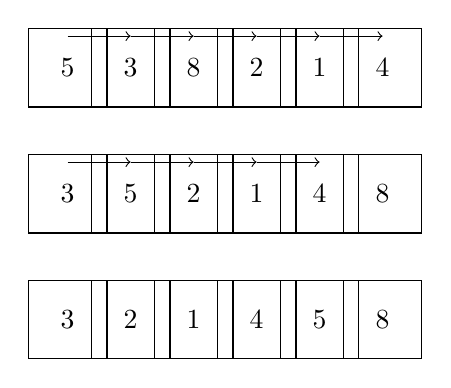
\begin{tikzpicture}[scale=0.8]
    \foreach \x/\val [count=\i] in {1/5,2/3,3/8,4/2,5/1,6/4} {
        \node at (\x,0) [draw, rectangle, minimum width=1cm, minimum height=1cm] {\val};
    }
    
    \foreach \i in {1,...,5} {
        \pgfmathtruncatemacro{\j}{\i+1}
        \draw[->] (\i,0.5) -- (\j,0.5);
    }
    
    \foreach \x/\val [count=\i] in {1/3,2/5,3/2,4/1,5/4,6/8} {
        \node at (\x,-2) [draw, rectangle, minimum width=1cm, minimum height=1cm] {\val};
    }
    
    \foreach \i in {1,...,4} {
        \pgfmathtruncatemacro{\j}{\i+1}
        \draw[->] (\i,-1.5) -- (\j,-1.5);
    }
    
    \foreach \x/\val [count=\i] in {1/3,2/2,3/1,4/4,5/5,6/8} {
        \node at (\x,-4) [draw, rectangle, minimum width=1cm, minimum height=1cm] {\val};
    }
\end{tikzpicture}


\subsection{Pseudocode}


\begin{algorithm}[H]
\captionsetup{justification=centering}
\caption{Bubble Sort}
\begin{algorithmic}[1]
\Procedure{BubbleSort}{$A$}
    \State $n \gets \text{length of } A$
    \For{$i \gets 0$ to $n-1$}
        \For{$j \gets 0$ to $n-i-1$}
            \If{$A[j] > A[j+1]$}
                \State swap $A[j]$ and $A[j+1]$
            \EndIf
        \EndFor
    \EndFor
\EndProcedure
\end{algorithmic}
\end{algorithm}



\subsection{Time and Space Complexity}


\textbf{Time Complexity}:
\begin{itemize}
    \item \textbf{Best Case}: $O(n)$ - when the input list is already sorted, and no swaps are needed.
    \item \textbf{Average Case}: $O(n^2)$ - on average, bubble sort requires $n^2/2$ comparisons and swaps.
    \item \textbf{Worst Case}: $O(n^2)$ - when the input list is sorted in reverse order, and each pair of elements needs to be swapped.
\end{itemize}


\textbf{Space Complexity}:
\begin{itemize}
    \item $O(1)$ - Bubble sort has a space complexity of $O(1)$ as it only requires a constant amount of extra space for temporary variables during the swapping process.
\end{itemize}


\subsection{Practical Applications}

Bubble sort can be used in situations where simplicity and ease of implementation are more important than efficiency:
\begin{itemize}
       \item It can be used for sorting small arrays or lists where the number of elements is relatively small. 
       \item  Bubble sort is a stable sorting algorithm, meaning that it preserves the relative order of equal elements. If stability is a requirement, bubble sort can be used in such cases.
\end{itemize}


\section{Heap Sort}

Heap sort is a comparison-based sorting algorithm. It divides its input into a sorted and an unsorted region, and it iteratively shrinks the unsorted region by extracting the largest element from it and inserting it into the sorted region. Heapsort does not waste time with a linear-time scan of the unsorted region; rather, heap sort maintains the unsorted region in a heap data structure to efficiently find the largest element in each step.

The heap Sort algorithm begins by rearranging the array into a binary max-heap. The algorithm then repeatedly swaps the root of the heap (the greatest element remaining in the heap) with its last element, which is then declared to be part of the sorted suffix. Then the heap, which was damaged by replacing the root, is repaired so that the greatest element is again at the root. This repeats until only one value remains in the heap.



\subsection{Pseudocode}


\begin{algorithm}[H]
\captionsetup{justification=centering}
\caption{Heap Sort}
\begin{algorithmic}
\Function{HeapSort}{$arr, n$}
    \State \Call{BuildHeap}{$arr, n$}
    \For{$i \gets n$ to $2$}
        \Call{Swap}{$arr[1], arr[i]$}
        \State $n \gets n - 1$
        \Call{Heapify}{$arr, 1, n$}
    \EndFor
\EndFunction


\Function{BuildHeap}{$arr, n$}
    \For{$i \gets n/2$ downto $1$}
        \Call{Heapify}{$arr, i, n$}
    \EndFor
\EndFunction


\Function{Heapify}{$arr, i, n$}
    \State $largest \gets i$
    \State $l \gets 2i$
    \State $r \gets 2i + 1$
    \If{$l \leq n$ \textbf{and} $arr[l] > arr[largest]$}
        \State $largest \gets l$
    \EndIf
    \If{$r \leq n$ \textbf{and} $arr[r] > arr[largest]$}
        \State $largest \gets r$
    \EndIf
    \If{$largest \neq i$}
        \Call{Swap}{$arr[i], arr[largest]$}
        \Call{Heapify}{$arr, largest, n$}
    \EndIf
\EndFunction


\Function{Swap}{$a, b$}
    \State $temp \gets a$
    \State $a \gets b$
    \State $b \gets temp$
\EndFunction
\end{algorithmic}
\end{algorithm}

 
\subsection{Time and Space Complexity}


\textbf{Time Complexity}:
\begin{itemize}
    \item Heap sort has a time complexity of $O(n log n)$ for the best, average and worst case scenarios. This is because the heapify operation takes $O(log n)$ time and it needs to be performed for each element in the array, resulting in a total time complexity of $O(n log n)$. 
\end{itemize}


\textbf{Space Complexity}:
\begin{itemize}
    \item The space complexity of heap sort is $O(1)$ as it operates in place and does not require any additional space other than the input array
\end{itemize}


\subsection{Practical Applications}


Applications of Heap Sort include:
\begin{itemize}
       \item Sorting large datasets: Heap sort is efficient for sorting large datasets due to its $O(n log n)$ time complexity.
       \item External sorting: Heap sort can be used for external sorting where the data is too large to fit into memory and needs to be sorted using disk-based algorithms.
\end{itemize}


\section{Quick Sort}
Quicksort is an efficient, general-purpose sorting algorithm. 
Quicksort is a divide-and-conquer algorithm. 
It works by selecting a 'pivot' element from the array and partitioning the other elements into two sub-arrays,
according to whether they are less than or greater than the pivot. 
For this reason, it is sometimes called partition-exchange sort.
The sub-arrays are then sorted recursively. This can be done in-place, 
requiring small additional amounts of memory to perform the sorting.


\begin{figure}[H]

    \QSinitialize{6, 5, 3, 1, 8, 7}

    \textbf{Step 1:} Choose a pivot
    
    \QSpivotStep
    \smallskip
    
    \textbf{Step 2:} Lesser values go to the left, equal or greater values go to the right
    
    \QSsortStep
    \smallskip
    
    \textbf{Step 3:} Repeat step 1 with the two sub lists
    
    \QSpivotStep
    \smallskip
    
    \textbf{Step 4:} Repeat step 2 with the sub lists:
    
    \QSsortStep
    \smallskip
    
    \textbf{Step 5:} and again and again!
    
    \loop
    \QSpivotStep
    \ifnum\value{pivotcount}>0
      \QSsortStep
    \repeat

  \caption{The operation of QUICK-SORT on the array 
  $A = \langle6, 5, 3, 1, 8, 7 \rangle $. }

\end{figure}


\subsection{Pseudocode}

\begin{algorithm}[H]
  \captionsetup{justification=centering}
  \caption{Quick Sort}
\begin{algorithmic}[1]
  \State \textbf{QuickSort}(A):
  \If {$ A.length < 1$}
    \State choose a pivot
    \While{ (there are items left in the array) }
    \If {$item < pivot $}
      \State put item in subarray1
    \Else 
      \State put item in subarray2
    \EndIf
    \EndWhile
  \State QuickSort(subarray1)
  \State QuickSort(subarray2)
  \EndIf
\end{algorithmic}
\end{algorithm}


\subsection{Time and Space Complexity}

\textbf{Time Complexity}:
\begin{itemize}
    \item \textbf{Best Case}: $O(n \log n)$ - The scenario occurs when the pivot divides the array into two nearly equal halves, leading to well-balanced partitioning.
    \item \textbf{Average Case}: $O(n \log n)$ - This scenario considers all possible cases and calculates the average time complexity. Moreover, it's assumed that all permutations of array element orders are equally likely.
    \item \textbf{Worst Case}: $O(n^2)$ - The worst-case scenario occurs when the smallest or largest element is chosen as a pivot. In this case, the partitioning is heavily unbalanced, leading to significantly higher time complexity.
\end{itemize}

\textbf{Space Complexity}:
\begin{itemize}
    \item $O(\log n)$ - Quicksort has a space complexity of $O(\log n)$ in the average case. 
    This arises from the recursive function calls and the partitioning process. It can be $O(n)$ 
    due to an unbalanced partitioning leading to a deep recursion stack in the worst case.
\end{itemize}

\subsection{Practical Applications}

Quick Sort is particularly useful when:
\begin{itemize}
    \item It is used everywhere where a stable sort is not needed.
    \item The sorting algorithm is used for information searching 
    and as Quicksort is the fastest algorithm so it is widely used as a better way of searching.
\end{itemize}





\section{ Related Works}

Sorting algorithms have been extensively studied, leading to various methods 
optimized for different data and computing environments. This section reviews 
key developments in Mergesort, Heapsort, Quicksort, Insertionsort, and Bubblesort, 
focusing on their theoretical foundations and practical implementations.
\begin{itemize}
  \item \textbf{Insertionsort}:Insertionsort is a simple algorithm with 
  $(O(n^2))$ average and worst-case time complexity but performs 
  well with $(O(n))$ complexity for nearly sorted arrays. It is stable and efficient 
  for small datasets and is often used as a subroutine in more complex 
  algorithms (Knuth, 1997; Cormen et al., 2009).
  \item \textbf{Mergesort}:Introduced by John von Neumann in 1945, 
  Mergesort is a divide-and-conquer algorithm with a time complexity of $(O(n \log n))$. 
  It is stable and efficient for large datasets but has an $(O(n))$ space complexity, 
  which can be a drawback (Cormen et al., 2009; Knuth, 1997).
  \item \textbf{Bubblesort}:Bubblesort, known for its simplicity, 
  has an $(O(n^2))$ time complexity, making it impractical for 
  large datasets. It is primarily used for educational purposes 
  to illustrate basic sorting concepts (Knuth, 1997; Sedgewick, 2002).
  \item \textbf{ Heapsort}:Developed by J. W. J. Williams in 1964, Heapsort transforms 
  the array into a binary heap, operating in $(O(n \log n))$ time and $(O(1))$ space. 
  It is efficient for memory-constrained environments but is less stable and often slower 
  than Quicksort in practice (Williams, 1964; Sedgewick, 2002).
  \item \textbf{Quicksort}: Tony Hoare's Quicksort (1960) is renowned for its 
  average-case $(O(n \log n))$ time complexity and high practical performance. 
  Despite its worst-case $(O(n^2))$ complexity, optimizations like 
  randomized partitioning enhance its efficiency (Hoare, 1962; Musser, 1997).
  \item \textbf{Comparative Analyses}Studies comparing these algorithms, 
  such as those by Bentley and McIlroy (1993) and Sedgewick (2002), 
  provide insights into their performance and optimizations. 
  Recent work by LaMarca and Ladner (1999) examines cache performance, 
  highlighting the practical implications of algorithmic choices in modern computing.
\end{itemize}



\section{Conclusion}

\begin{table}[H]
  \begin{tabular}{@{}lllll@{}}
  \toprule
  Algorithms & Time Complexity         & Space Complexity \\ \midrule
  Insertion sort     & $O(n^2)$             &$O(1)$ \\
  Merge sort         & $O(n \log n)$        & $O(n)$ \\
  Bubble sort        & $O(n^2)$             & $O(1)$ \\
  Heap sort          & $O(n \log n)$        & $O(1)$ \\
  Quick sort         & $O(n \log n)$        & $O(n)$ \\ \bottomrule
  \end{tabular}
  \end{table}

  In conclusion, sorting algorithms play a fundamental role in computer science, 
  serving as critical tools for organizing data efficiently. 
  Each of the discussed algorithms( mergesort, heapsort, quicksort, 
  insertionsort, and bubblesort )offers unique advantages and limitations 
  that make them suitable for different scenarios and data sets.
  \newline
  Mergesort, with its stable and predictable $O(n \log n)$ performance, 
  is ideal for large datasets and is well-suited for external sorting due 
  to its consistent splitting and merging approach. Heapsort, also with $O(n \log n)$ 
  complexity, is notable for its in-place sorting and good worst-case performance, 
  making it valuable in memory-constrained environments.
  
  Quicksort is often preferred in practice due to its average-case 
  efficiency and cache-friendly nature, despite its $O(n^2)$ worst-case 
  scenario, which can be mitigated with good pivot selection strategies 
  like median-of-three. Insertionsort, while inefficient for large datasets 
  with its $O(n^2)$ complexity, excels with small or nearly sorted arrays due 
  to its simplicity and low overhead. 
  Bubblesort, although largely impractical for serious applications due to its 
  $O(n^2)$ complexity, serves as an educational tool for understanding basic 
  algorithmic principles.
  
  In practical applications, the choice of sorting algorithm is heavily influenced 
  by the specific requirements of the task at hand, including the size of the dataset, 
  memory constraints, and the need for stability. Understanding the underlying mechanics 
  and performance implications of each algorithm enables informed decisions that optimize 
  both efficiency and resource utilization in software development.
  
  By comprehensively evaluating these sorting algorithms, we appreciate 
  the diverse strategies employed in data organization and the continuous 
  evolution of algorithmic design, highlighting the significance of both 
  theoretical knowledge and practical application in computer science.
%%
%% The next two lines define the bibliography style to be used, and
%% the bibliography file.
\bibliographystyle{ACM-Reference-Format}
\bibliography{mybib}


\end{document}
\endinput
%%